% =====================================================================================
% REVISIÓN 2  -  Propuesta de solución
% Escribe tu texto FUERA de los recuadros \begin{guia} ... \end{guia}.
% =====================================================================================

\section{Propuesta de solución} \label{sec:propuesta} % audit:req=propuesta_solucion

\begin{guia}[Guía: Propuesta de solución (Revisión 2)]
\textbf{¿Para qué sirve?} Explica \emph{qué vas a hacer exactamente y cómo resuelve el problema}, antes de entrar a los
detalles de construcción (Revisión 3).

\textbf{Debe responder:}
\begin{itemize}[nosep,leftmargin=*]
  \item ¿En qué consiste la solución, a grandes rasgos? Incluye un diagrama general (arquitectura, flujo del proceso o
        esquema del método).
  \item \emph{Proyecto de sistema:} ¿cuáles son los requisitos funcionales (qué hará) y no funcionales (rendimiento,
        seguridad, usabilidad)? ¿quiénes son los usuarios y qué roles tienen?
  \item \emph{Proyecto de investigación:} ¿cuál es la hipótesis o pregunta de investigación? ¿qué enfoque o algoritmo
        propones y en qué se diferencia de lo existente?
  \item ¿Qué tecnologías, herramientas y metodología de trabajo usarás y por qué (frente a las alternativas)?
  \item ¿Cómo atiende la propuesta cada objetivo específico? (una tabla ``objetivo $\rightarrow$ componente de la solución''
        es muy útil).
  \item ¿Cuál es el plan de trabajo y el cronograma del cuatrimestre?
  \item ¿Cómo sabrás que funcionó? (criterios de aceptación o métricas de éxito).
\end{itemize}

\textbf{Organización sugerida:} \verb|\subsection| para \emph{Descripción general}, \emph{Requisitos} (o \emph{Hipótesis y
enfoque}), \emph{Tecnologías y metodología} y \emph{Plan de trabajo}.

\textbf{Extensión mínima:} 150 palabras, además de diagramas y tablas.

\textbf{Errores frecuentes:} describir solo tecnologías sin explicar la solución; requisitos vagos (``el sistema será
rápido''); propuesta desconectada de los objetivos; cronograma sin fechas.

\textbf{Cómo se revisa:} coherencia con el problema y los objetivos, viabilidad en un cuatrimestre y claridad técnica.
\end{guia}

% >>> ESCRIBE AQUÍ la propuesta de solución (con una \subsection por apartado) <<<
\subsection{Descripción general}

La propuesta consiste en realizar un estudio comparativo de Grandes Modelos de Lenguaje de 1-bit identificados a partir de la literatura científica. El trabajo parte de la revisión de conceptos relacionados con los Grandes Modelos de Lenguaje, los modelos de 1-bit y las métricas utilizadas para evaluar este tipo de propuestas.

Posteriormente, se analizará cada uno de los modelos seleccionados con el propósito de conocer sus principales características, su funcionamiento, la forma en que son entrenados, el tipo de representación utilizada para sus pesos y los resultados que reportan sus respectivos trabajos científicos.

A partir de esta información se establecerán las métricas y criterios que permitirán realizar una comparación entre los modelos. Para ello, se utilizará una matriz en la que se relacionen los modelos seleccionados con las distintas métricas consideradas, permitiendo identificar qué información de evaluación se encuentra disponible para cada propuesta.

Después se realizarán pruebas sobre los modelos utilizando las mismas preguntas para cada uno, con el propósito de obtener resultados comparables. A partir de las respuestas obtenidas, los modelos serán evaluados mediante las métricas y criterios definidos previamente. Finalmente, los resultados serán discutidos para identificar las principales diferencias, ventajas y limitaciones de cada modelo, así como determinar cuál presenta las mejores condiciones para continuar trabajando con él en etapas posteriores cercanas.


\subsection{Pregunta de investigación y enfoque}

\textbf{Pregunta de investigación.}

Mediante las mismas preguntas y las mismas pruebas, ¿Cuál de los modelos seleccionados resulta la mejor opción y por qué?

\textbf{Enfoque.}

Aunque los modelos pueden compararse utilizando métricas comunes, determinar que uno de ellos es la mejor opción de manera general puede no representar correctamente sus características. Cada modelo puede presentar ventajas o limitaciones dependiendo del objetivo, las condiciones de uso y los recursos disponibles. Por esta razón, el análisis no se limitará a identificar un único modelo como superior, sino que buscará determinar en qué condiciones o enfoques cada propuesta puede resultar más adecuada.


\subsection{Tecnologías y metodología}

La parte experimental se realizará en un entorno orientado a dispositivos móviles mediante un emulador de Android. Antes de comenzar las pruebas se definirá un conjunto fijo de consultas que será utilizado durante las ejecuciones, con el propósito de mantener una condición común de evaluación.

Para cada implementación se seguirá una misma estructura de trabajo: preparación del modelo, ejecución de las consultas definidas, registro de las respuestas y medición de las métricas correspondientes. Además, se conservarán evidencias de cada ejecución mediante capturas de pantalla, de manera que los resultados puedan revisarse posteriormente durante la etapa de análisis.

Las herramientas específicas de implementación, como el emulador, lenguaje, librerías o framework, se definirán conforme avance el proyecto y de acuerdo con los requisitos técnicos de cada modelo.


\subsection{Relación con los objetivos específicos}

La relación entre los objetivos específicos y la propuesta se muestra en la Tabla~\ref{tab:relacion_objetivos}.

\begin{table}[H]
\centering
\small
\caption{Relación entre los objetivos específicos y la propuesta}
\label{tab:relacion_objetivos}

\begin{tabular}{L{5.8cm} L{8.2cm}}
\toprule
\textbf{Objetivo específico} & \textbf{Relación} \\
\midrule

Obtener 1 compendio de la documentación de los 1-bit LLM de la literatura.
&
Este objetivo se desarrollará a partir de la búsqueda, revisión y organización de información proveniente de la literatura científica sobre los modelos seleccionados.
\\
\midrule

Establecer 1 conjunto de criterios de selección de los 1-bit LLM de la literatura.
&
Para cumplirlo se definirán métricas y criterios que permitan analizar las características de los modelos y establecer una base común de comparación.
\\
\midrule

Implementar los 5 mejores 1-bit LLM.
&
La propuesta contempla preparar e implementar los modelos seleccionados con el fin de poder ejecutarlos y realizar las pruebas correspondientes.
\\
\midrule

Obtener 1 repositorio de datos para probar los 1-bit LLM seleccionados.
&
Se organizará un conjunto de consultas que pueda utilizarse de forma consistente durante las pruebas de los modelos.
\\
\midrule

Comparar los 5 1-bit LLM seleccionados.
&
Los resultados obtenidos durante las ejecuciones serán registrados y analizados utilizando métricas comunes, con el propósito de identificar diferencias entre las propuestas.
\\

\bottomrule
\end{tabular}
\end{table}


\subsection{Plan de trabajo y cronograma}

El trabajo se organizará por etapas tomando como referencia el avance real desarrollado durante el cuatrimestre.

\textbf{Etapa 1. Primer mes:} se trabajó en comprender los conceptos básicos relacionados con los Grandes Modelos de Lenguaje, los modelos de 1-bit y algunas de las propuestas existentes dentro de esta línea de investigación.

\textbf{Etapa 2. Segundo mes:} se profundizó en el estudio de los modelos seleccionados, analizando de manera individual su funcionamiento, método de entrenamiento, características principales y los resultados que busca conseguir cada propuesta.

\textbf{Etapa 3. Mes actual:} se continuará con la comparación de los modelos mediante pruebas, consultas y métricas comunes, con el propósito de identificar sus diferencias y determinar cuáles presentan mejores condiciones para continuar con el trabajo experimental.

\textbf{Etapa 4. Antes de finalizar el cuatrimestre:} se contará con un modelo seleccionado a partir de los resultados obtenidos y con una implementación funcional que permita continuar trabajando con él en etapas posteriores.


\subsection{Criterios de éxito o métricas}

Los modelos serán evaluados con las mismas consultas y bajo el mismo procedimiento. Para compararlos se utilizarán métricas como perplejidad, exactitud, tamaño del modelo, memoria, latencia, velocidad, bits por peso y compresión.

Con los resultados obtenidos se comparará el desempeño de cada modelo y se descartarán las opciones menos favorables según los criterios definidos. Finalmente, se identificarán los modelos que presenten mejores condiciones para continuar con el proyecto.


\subsection{Diagrama general del proceso}

El proceso general de la propuesta se muestra en la Figura~\ref{fig:diagrama_propuesta}.

\begin{figure}[H]
    \centering
    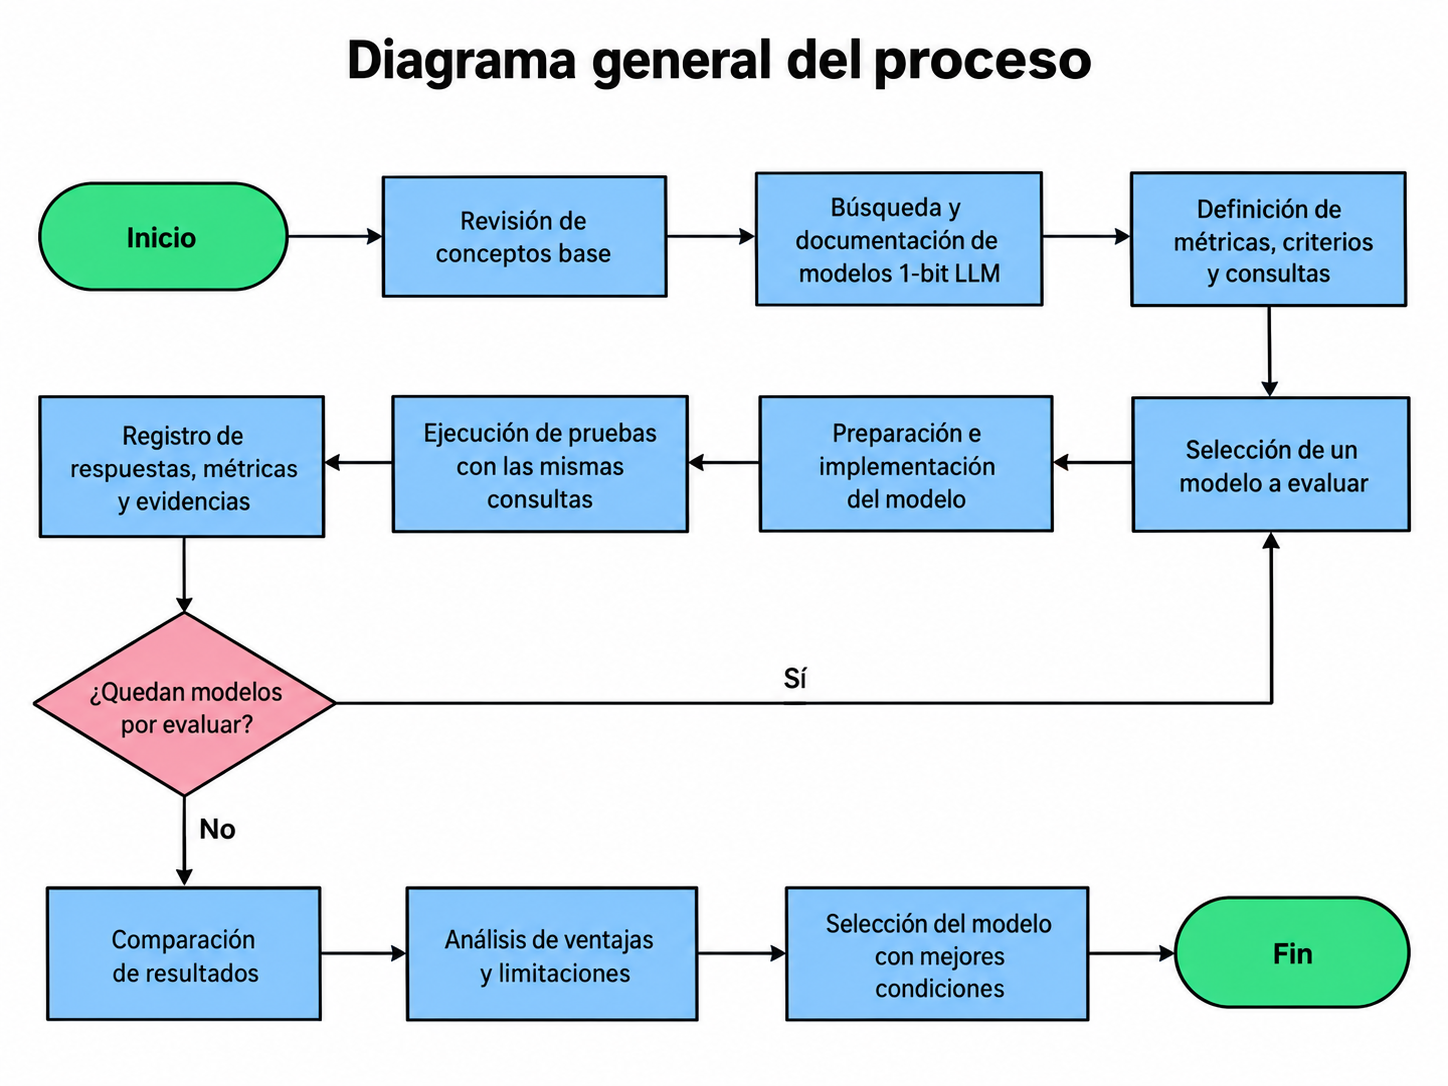
\includegraphics[width=0.95\textwidth]{img/DiagramaGeneral.png}
    \caption{Diagrama general del proceso de la propuesta}
    \label{fig:diagrama_propuesta}
\end{figure}
